
\documentclass[a4paper,12pt]{article}
\usepackage{amsmath}
\usepackage{amssymb}
\usepackage[polish]{babel}
\usepackage{polski}
\usepackage[utf8]{inputenc}
\usepackage{indentfirst}
\usepackage{geometry}
\usepackage{array}
\usepackage[pdftex]{color,graphicx}
\usepackage{subfigure}
\usepackage{afterpage}
\usepackage{setspace}
\usepackage{color}
\usepackage{wrapfig}
\usepackage{listings}
\usepackage{datetime}

\renewcommand{\onehalfspacing}{\setstretch{1.6}}

\geometry{tmargin=2.5cm,bmargin=2.5cm,lmargin=2.5cm,rmargin=2.5cm}
\setlength{\parindent}{1cm}
\setlength{\parskip}{0mm}

\newenvironment{lista}{
\begin{itemize}
  \setlength{\itemsep}{1pt}
  \setlength{\parskip}{0pt}
  \setlength{\parsep}{0pt}
}{\end{itemize}}

\newcommand{\linia}{\rule{\linewidth}{0.4mm}}

\definecolor{lbcolor}{rgb}{0.95,0.95,0.95}
\lstset{
    backgroundcolor=\color{lbcolor},
    tabsize=4,
  language=C++,
  captionpos=b,
  tabsize=3,
  frame=lines,
  numbers=left,
  numberstyle=\tiny,
  numbersep=5pt,
  breaklines=true,
  showstringspaces=false,
  basicstyle=\footnotesize,
  identifierstyle=\color{magenta},
  keywordstyle=\color[rgb]{0,0,1},
  commentstyle=\color{blue},
  stringstyle=\color{red}
  }

\begin{document}

\noindent
\begin{tabular}{|c|p{11cm}|c|} \hline 
Grupa 4 & Barbara Nowak, Piotr Tomaszewski & \ddmmyyyydate\formatdate{26}{10}{2016} \tabularnewline
\hline 
\end{tabular}


\section*{Zadanie 4 - Rozmycie Gaussa w OpenMP}
Celem naszego zadania było zaimplementowanie programu rozmywającego wybrane zdjęcie za pomocą algorytmu Gaussa z maską o wymiarach 5x5. Do zrównoleglenia obliczeń wykorzystaliśmy bibliotekę OpenMP.

Program uruchamiany jest z dwoma argumentami: \quotedblbase ilWatkow \textquotedblright - to liczba wątków a pozostałe dwa to odpowiednio lokalizacja pliku źródłowego oraz ścieżka do zapisu zmodyfikowanego pliku. Początkowo sprawdzamy poprawności wprowadzanych danych.
Kolejnym krokiem jest wczytanie pliku do zmiennej \quotedblbase zdjecie \textquotedblright typu \quotedblbase Mat \textquotedblright za pomoca funkcji imread. 
\begin{lstlisting}
zdjecie = imread(argv[2], CV_LOAD_IMAGE_COLOR);
\end{lstlisting}
Następnie deklarujemy maskę w postaci 2 - wymiarowej tablicy liczb całkowitych, o wymiarach 5x5. Za pomocą funkcji smasek obliczamy sume masek, która jest niezbędna do prawidłowego wykonania rozmycia Gaussa na wczytanum obrazku.

\begin{lstlisting}
int sMasek(int maska[5][5], int i, int j)
{
	int suma=0;	
	for(i = 0; i < 5; ++i)
	{
        for(j = 0; j < 5; ++j)
		{
			suma += maska[i][j];		//Musi byc rozna od 0!
		}
	}
	return suma;
}
\end{lstlisting}

Tworzymy kopię wczytanego obrazka za pomocą funkcji \quotedblbase clone() \textquotedblright. Kolejnym krokiem jest ustawienie liczby watków dla zrównoleglonych obszarów. 
\begin{lstlisting}
omp_set_num_threads(ilWatkow); 
\end{lstlisting}

Etapem końcowym jest zapisanie zmodyfikowanego obrazu do ścieżki z argumentu argv[3] za pomocą funkcji imwrite(), która jako pierwszy argument przyjmuje ścieżkę docelową, a drugim argumentem jest funkcja \quotedblbase rozmycie() \textquotedblright która rozmywa nasz obrazek za pomocą algorytmu Gaussa z maską 5x5.
\begin{lstlisting}
imwrite(argv[3], rozmycie(sumaMasek,zdjecieKopia,zdjecie, maska));
\end{lstlisting}
W funkcji rozmycie() pierwszą czynnością jaką wykonujemy jest uruchomienie pomiaru czasu, następnie stosujemy procedurę zrónoleglania OpenMP w celu przyspieszenia obliczen.
\begin{lstlisting}
#pragma omp parallel for default(shared) private(i,j,k,l,zmPiksel,r,g,b,zmI,zmJ)
\end{lstlisting}
Powyższa dyrektywa zawiera następujące parametry: parallel - wskazanie kompilatorowi obszaru kodu, który będzie zrównoleglany, omp - słowo kluczowe odnoszące się do OpenMP, for - informuje że zrównoleglana będzie pętla for, default(shared)  utawienie zasiegu zmiennych wewnatrz rownolegle przetwarzanego obszaru, 
(gdzie parametr "shared" powoduje, ze domyslnie wszystkie zmienne w petli sa wspolne), private (...) - okreslenie zmiennych prywatnych (do ktorych tylko jeden wątek ma dostep.

Następnie poruszając się po wierszach i kolumnach wczytanego obrazka, nawigujemy aby wspolrzedne tymczasowe nie wykroczyly poza obraz. Pobieramy wartosci każdego pixela w postaci 3 bitowego wektora (RGB)	by następnie obliczyć dla niego nową wartość, kontrolując wartości by nie wyszły poza zakres [0 - 255].


\begin{lstlisting}
// pobranie wartosci pixela w postaci 3 bitowego wektora (RGB)
zmPiksel = zdjecie.at<Vec3b>(Point(zmI, zmJ));					
...
r+=zmPiksel.val[0]*maska[i][j];
g+=zmPiksel.val[1]*maska[i][j];
b+=zmPiksel.val[2]*maska[i][j];
...
((r/sumaMasek)>255)? (r=255) : (r=r/sumaMasek);
((g/sumaMasek)>255)? (g=255) : (g=g/sumaMasek);
((b/sumaMasek)>255)? (b=255) : (b=b/sumaMasek);
\end{lstlisting}
 Pod koniec nanosimy nowe wartości pixeli RGB.
\begin{lstlisting}
zdjecieKopia.at<Vec3b>(Point(l,k))=Vec3b(r,g,b);		
\end{lstlisting}

\begin{wrapfigure}{r}{0.5\textwidth}
	\vspace{-40pt}
	\begin{center}
		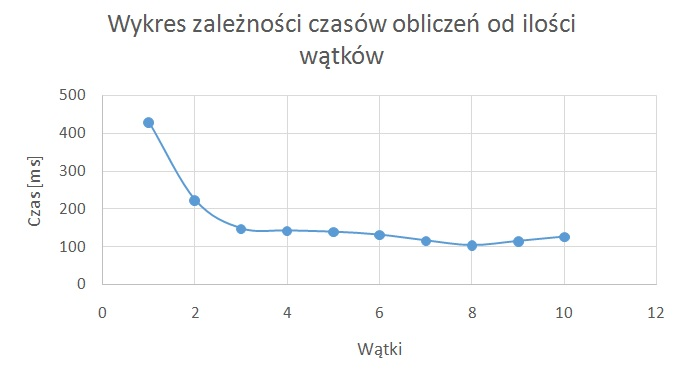
\includegraphics[width=0.5\textwidth]{img1.jpg}
	\end{center}
	\vspace{-20pt}
	\caption{Wykres zależności czasu obliczeń od liczby wątków}
	\vspace{35pt}
\end{wrapfigure}

Wykres zależności czasów obliczeń od ilości wątków (Rysunek 1) ukazuje, że ze wzrostem liczby wątków czas obliczeń znacznie spada. Przy czterech wątkach czas lekko wzrasta, potem płynnie opada aż do 8 wątków, po osiągnięciu których znów wzrasta. 

Zrównoleglenie przy użyciu OpenMP obrazuje poniższy wykres przyspieszenia od ilości watków (Rysunek 2). Program przyspiesza do  ośmiu wątków a następnie zwalnia. Serwer uruchomieniowy ma 4-rdzeniowy procesor z technologią Hyper-Threading dlatego przy większej ilości wątków niż ma procesor, czas lekko rośnie.

\begin{wrapfigure}{r}{0.5\textwidth}
	\vspace{-40pt}
	\begin{center}
		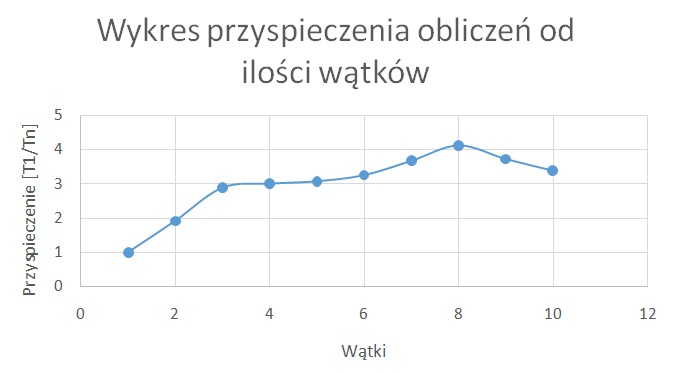
\includegraphics[width=0.5\textwidth]{img2.jpg}
	\end{center}
	\vspace{-20pt}
	\caption{Wykres przyspieszenia}
	\vspace{35pt}
\end{wrapfigure}


\textbf{Podsumowanie:} OpenMP to rozszerzenie dla języków C/C++ pozwalające mieć wpływ na programowanie wielowątkowe. Każdy z wątków może posiadać własny tymczasowy widok na wspólny obszar pamięci. Zmienne zawarte w bloku parallel można podzielić na private - zmienne do których tylko jeden wątek ma dostęp i shared - dostęp wielu wątków do zmiennych. Używanie większej ilości wątków niż jest to sprzętowo możliwe to nie najlepsze rozwiązanie. Można pomyśleć, że przy nieskończonej ilości wątków czas będzie dążył do zera - to nie jest prawda. Po przekroczeniu możliwości procesora, czas wykonywania programu wzrośnie. Algorytm Gaussa pozwolił nam w prosty i łatwy sposób dokonać rozmycia zadanej fotografii.

\end{document}
